
Beauty and the Burst~\cite{schuster2017beautyburst} uses Convolutional Neural Networks (CNNs) for video identification. 
CNNs have been shown to be effective in sequence modeling for decades~\cite{hinton1990connectionist}.
However, there are two problems with using a convolutional neural network as a sequence modeler.
First, convolutional layers applied to a sequence are not inherently causal, meaning that they look into future samples of a sequence to decide the output for the current sample.
Secondly, convolutional neural networks lack a deep effective history size of past samples in the sequence (i.e. their effective history is bounded to the number of samples that kernel can cover from the past).
To address these problems, Bai\etalc{bai2018empirical} proposed a new architecture called Temporal Convolutional Network (TCN).
The TCN utilizes a one-dimensional fully-convolutional network~\cite{long2015fully} equipped with causal dilated convolutions~\cite{oord2016wavenet}, allowing it to examine deep into the past to produce an output for the sequence at any given moment.
They added a generic residual block from input to output.
The architecture is shown in the \Cref{fig:tcn-arch}.
We evaluate the effectiveness of TCN model for network side-channel attacks in \Cref{sec:eval-empirical-privacy}.



\begin{figure}[t]
  \centering
  %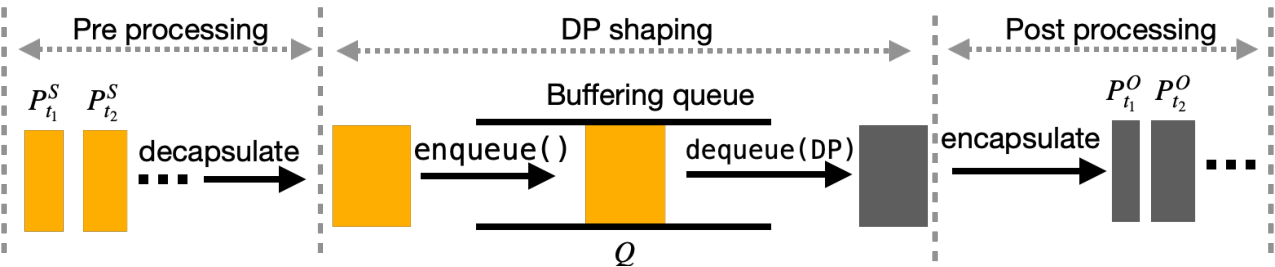
\includegraphics[width=\columnwidth]{figures/DPshaping_concept_vertical.pdf}
  %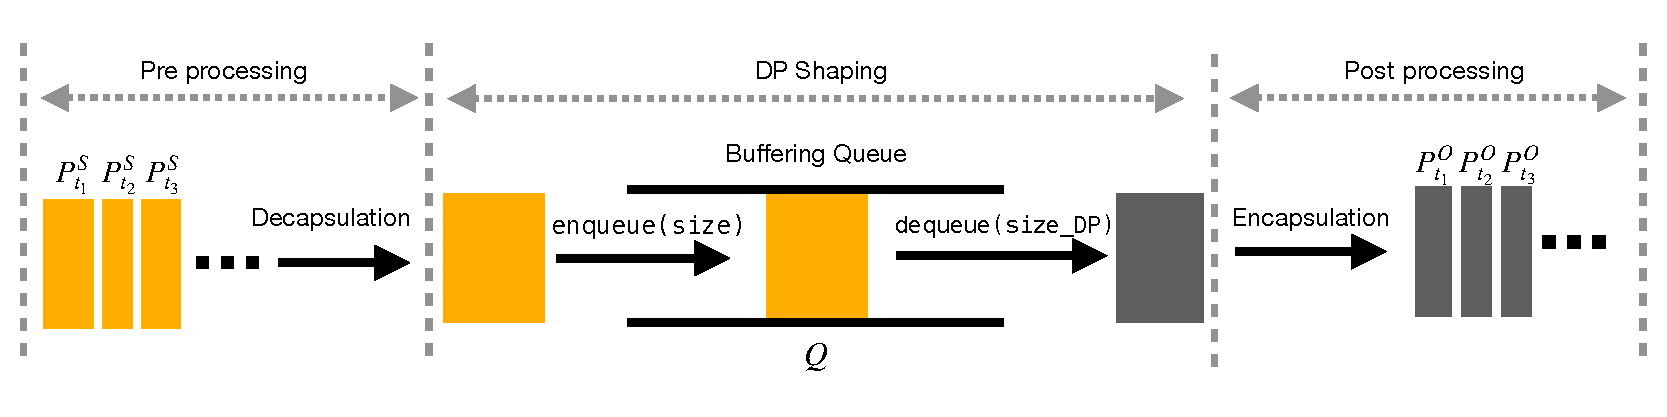
\includegraphics[width=\columnwidth]{figures/DPshaping_concept_horizontal.pdf}
  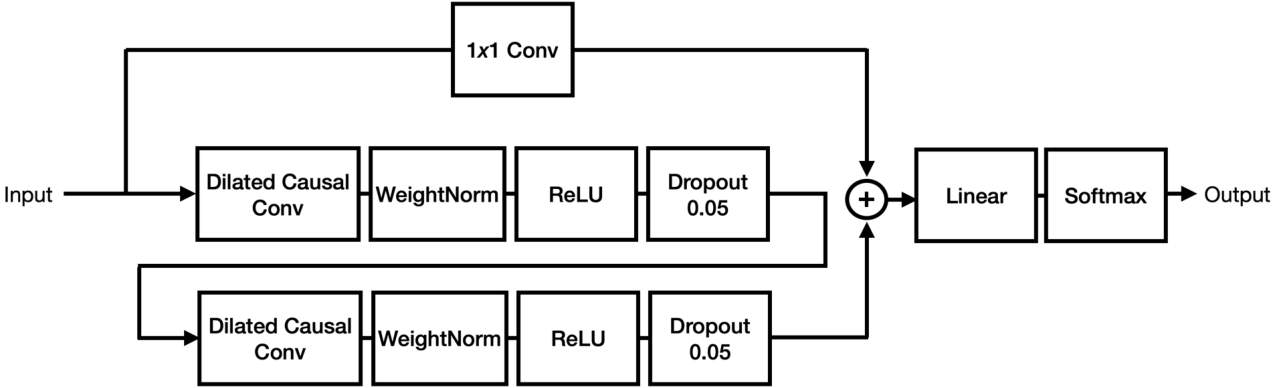
\includegraphics[width=\columnwidth]{figures/TCN_arch.pdf}
  \caption{TCN model architecture.}
  \label{fig:tcn-arch}
\end{figure}

